\documentclass{article}
\usepackage[a4paper,margin=1in,landscape]{geometry}
\usepackage{graphicx}
\usepackage{rotating}
\usepackage{siunitx}
\usepackage{multirow}
\usepackage{multicol}
\usepackage{pgfplotstable}
\usepackage{booktabs}
\sisetup{
		round-mode        = places,
		round-precision   = 2,
}
\begin{document}
		\title{Dumebi Valerie Duru}
		\maketitle
	\section{Logic Gates}
			Logic gates perform logical operations that take binary input (0s and 1s) and produce a single binary output. They are used in most electronic device including:
			\cite{hall2019opportunity}

	\begin{table}[h!]
		\begin{center}
			\caption{Logic Gates}
			\label{tab: table 1}
			\begin{tabular}{|c|c|c|}
					\hline
					Smartphones & Tablets & Memory Devices\\
					\hline
					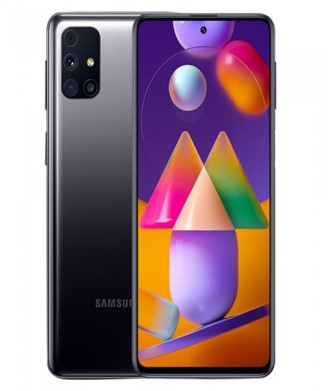
\includegraphics[width=0.1\linewidth]{phone.jpg} & 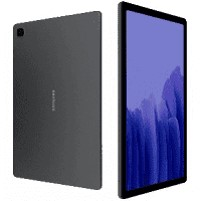
\includegraphics[width=0.1\linewidth]{tablet.jpg} &
					 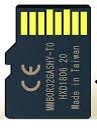
\includegraphics[width=0.1\linewidth]{memory device.jpg}\\
					\hline  			
			\end{tabular}
		\end{center}	
	\end{table}

	\begin{table}[h!]
		\caption{Multi row table}
		\label{tab: table 2}
		\begin{center}
		\begin{tabular}{|l|c|l|}
			\hline
			\textbf{Value 1} & \textbf{Value 2} & \textbf{Value 3}\\
			$\alpha$ & $\beta$ & $\gamma$\\ 
			\hline
			\multirow{2}{*}{12} & 1110.1 & a\\
			& 10.1 & b\\
			\hline
			14 & 25.11 & \multirow{2}{*}{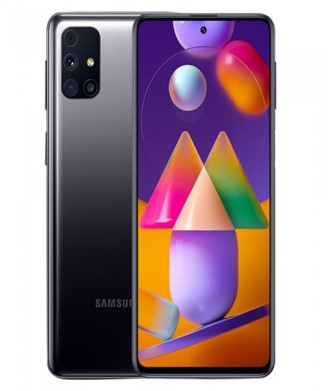
\includegraphics[width=0.05\linewidth]{phone.jpg}}\\
			25 & 345.113232 & \\
			\hline
			36 & 35.1234 & c\\
			\hline
			
		\end{tabular}
		\end{center}
	\end{table}

	\begin{table}[h!]
		\begin{center}
		\caption{Multicolumn table}
		\label{tab:table 3}
			\begin{tabular}{|l|c|r|}
				\hline
				\textbf{Value 1} & \textbf{Value 2} & \textbf{Value 3}\\
				$\alpha$ & $\beta$ & $\gamma$\\
				\hline
				\multicolumn{2}{|c|}{12} & a\\
				\hline
				2 & 10.1 & b\\
				3 & 23.1125 & c\\
				\hline
				\multicolumn{3}{|c|}{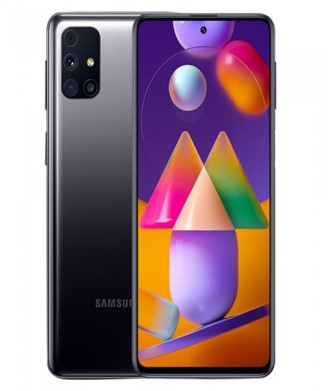
\includegraphics[scale=0.5]{phone.jpg}}\\
				\hline
				4 & 25.109 & d\\
				\hline
			\end{tabular}
		\end{center}
	\end{table}
	\newpage
	\bibliography{myBib.bib}
	\bibliographystyle{ieeetr}
	
	\begin{table}[h!]
		\caption{Autogenerated table}
		\label{table1}
		\pgfplotstabletypeset[multicolumn names, col sep=comma, display columns/0/.style={column name= $Dumebi 321$, column type={S},string type},
		display columns/1/.style = {column name = $Value$, column type = {S},string type}, every head row/.style={after row=\midrule},every last row/.style={after row=\bottomrule}]{table.csv}
		
		
	\end{table}
% Basic use of minipage environment



	
	Look at this text,
	\begin{minipage}{3cm}
		This text is processed in paragraph mode, and then becomes an indivisible \TeX{} box.
	\end{minipage}
	how strange!

\end{document}